\sezione{10}{Bayes con multinormali e superfici decisionali}{50–53}

Ora ogni classe ha la sua gaussiana $p(\x|w_i)$, con i propri $\mmu_i$ e $\SSigma_i$. La regola resta quella della sezione 2: in ogni punto vince la classe con $p(\x|w_i)P(w_i)$ più alto. Cambia la \emph{forma} del confine.

\subsection{Regioni e superfici decisionali}
\begin{intuizione}
Immagina due «montagne» sopra il piano delle feature, alte $p(\x|w_1)P(w_1)$ e $p(\x|w_2)P(w_2)$ (slide 50). Ogni punto del piano appartiene alla classe la cui montagna è più alta lì sopra. Il \key{confine di decisione} (\emph{decision boundary} o \emph{decision surface}) è la linea dove le due montagne hanno la stessa altezza: lì la classificazione è \textbf{ambigua}.
\end{intuizione}
Lo spazio viene suddiviso in regioni $\Re_i$ che \textbf{non devono essere connesse}: nell'esempio della slide 50, $\Re_2$ è formata da due pezzi separati e il confine è composto da due iperboli.

\begin{minipage}[c]{.5\linewidth}
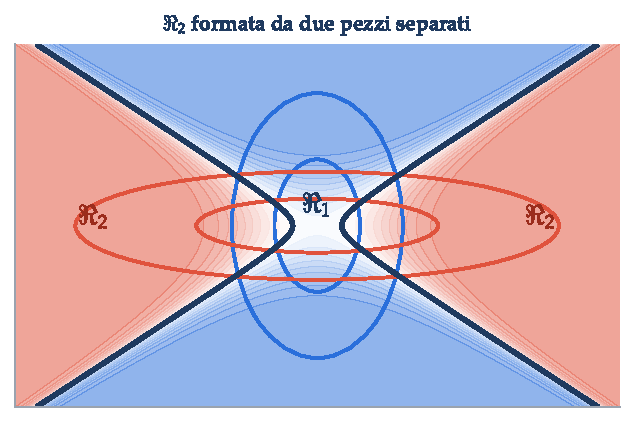
\includegraphics[width=\linewidth]{figs/regioni_disgiunte.pdf}
\end{minipage}\hfill
\begin{minipage}[c]{.46\linewidth}\raggedright
\small Due classi con la stessa media: la blu è più estesa in verticale, la rossa è lunga in orizzontale ma sottile. Sopra e sotto vince la blu, ai due lati la rossa. Il confine è formato da due \textbf{iperboli} e $\Re_2$ è spezzata in due regioni disgiunte, come nella slide 50.
\end{minipage}

\subsection{Le funzioni discriminanti}
\begin{tecnica}[Passare ai logaritmi]
Il logaritmo è crescente e non cambia l'argmax, quindi si può confrontare
\[
g_i(\x)=\ln p(\x|w_i)+\ln P(w_i)=-\frac12(\x-\mmu_i)\T\SSigma_i^{-1}(\x-\mmu_i)-\frac12\ln|\SSigma_i|-\frac d2\ln2\pi+\ln P(w_i)
\]
La decisione è $b=\argmax_i g_i(\x)$, e il confine tra $w_1$ e $w_2$ è l'insieme dei punti in cui $g_1(\x)=g_2(\x)$. Ogni $g_i$ è un polinomio di \textbf{secondo grado} in $\x$.
\end{tecnica}

\subsection{Caso 1: stessa matrice di covarianza → iperpiani}
Se $\SSigma_1=\SSigma_2=\SSigma$, sviluppando il prodotto il termine quadratico $\x\T\SSigma^{-1}\x$ è \textbf{uguale} in tutte le $g_i$ e si cancella nel confronto; si cancellano anche $\ln|\SSigma|$ e $\frac d2\ln2\pi$. Resta una funzione \textbf{lineare}:
\begin{formulat}{Covarianze uguali: discriminante lineare}
$\displaystyle g_i(\x)=\mathbf{w}_i\T\x+w_{i0},\qquad \mathbf{w}_i=\SSigma^{-1}\mmu_i,\qquad w_{i0}=-\frac12\mmu_i\T\SSigma^{-1}\mmu_i+\ln P(w_i)$
\end{formulat}
Il confine $g_1=g_2$ è quindi un \key{iperpiano}: un sottospazio di dimensione $d-1$ (una retta nel piano, un piano nello spazio 3D).

\subsection{Caso 2: covarianze arbitrarie → iperquadriche}
Se $\SSigma_1\neq\SSigma_2$ i termini quadratici \textbf{non} si cancellano: il confine è un'\key{iperquadrica}, una superficie descritta da un'equazione di secondo grado nelle coordinate (in 2D: ellissi, parabole, iperboli, coppie di rette).

\fig[.9\linewidth]{superfici.pdf}
\didascalia{Sfumatura = posteriori; linea scura = confine ($P=0.5$); ellissi = gaussiane delle classi. Sinistra e centro: stessa $\SSigma$, confine rettilineo che si sposta con il prior. Destra: covarianze diverse, confine curvo attorno alla classe più concentrata.}

\begin{esempio}[Cosa fa il prior (slide 52)]
Con $P(w_1)=P(w_2)=0.5$ la retta passa «a metà» tra le due classi. Con $P(w_1)=0.8$ e $P(w_2)=0.2$ la retta \textbf{si sposta verso $w_2$}: la classe più probabile conquista territorio. Il termine $\ln P(w_i)$ in $w_{i0}$ sposta l'iperpiano parallelamente a sé stesso, senza ruotarlo.
\end{esempio}
\begin{tecnica}[Il caso più semplice]
Con $\SSigma=\sigma^2I$ (classi sferiche e tutte uguali) e prior uguali, il confine è l'\textbf{asse del segmento} che unisce le due medie: si assegna $\x$ alla media più vicina in senso euclideo (classificatore a \emph{distanza minima}). Con $\SSigma$ generica ma uguale, «più vicina» va inteso in senso Mahalanobis.
\end{tecnica}
\begin{mlbox}[LDA e QDA]
Il caso 1 è la \textbf{Linear Discriminant Analysis} (LDA), il caso 2 la \textbf{Quadratic Discriminant Analysis} (QDA); in scikit-learn si chiamano proprio così. LDA ha meno parametri (una sola $\SSigma$ condivisa, stimata con i dati di tutte le classi) e rischia meno l'overfitting; QDA è più flessibile ma richiede più dati per classe. È di nuovo il compromesso bias-varianza della sezione 5.
\end{mlbox}

\begin{appunti}{— Sezione 10}
\pag{50} Densità condizionali «corrette» (moltiplicate) per i prior: $p(\x|w_i)P(w_i)$. In ogni punto vince la più alta.
\pag{51} Le regioni possono essere \textbf{non connesse} ($\Re_2$ in due pezzi). Boundary = zona ambigua ($P$ uguali). $g_i=\ln p(\x|w_i)+\ln P(w_i)$ quadratica in $\x$. $\SSigma$ uguali → \textbf{iperpiano}; $\SSigma$ arbitrarie → \textbf{iperquadrica}.
\pag{52} $\SSigma$ uguali: $x\T\SSigma^{-1}x$ si cancella, $g_i=\mathbf{w}_i\T\x+w_{i0}$. Iperpiano = dimensione $d-1$. Il prior sposta la retta verso la classe meno probabile (0.8/0.2). $\SSigma=\sigma^2I$: distanza minima dalle medie. = \textbf{LDA}.
\pag{53} $\SSigma$ diverse: equazione di 2° grado, ellissi/parabole/iperboli. = \textbf{QDA}.
\end{appunti}
